\documentclass[a4paper]{article}

\usepackage[english]{babel}
\usepackage[utf8]{inputenc}
\usepackage{amsmath}
\usepackage{graphicx}
\usepackage[colorinlistoftodos]{todonotes}
\usepackage{pdfpages}
\usepackage{alltt}

\title{Concepts Avancés de Bases de données}

\author{Joaquim LEFRANC et Jérôme SKODA}

\date{\today}

\begin{document}
\maketitle


\section{Nouveauté depuis le TP6}

\begin{itemize}
  \item Make gen-tp7 : Génération du fichier R du tp7 (necessite python3)
  \item Make demo-tp7 : Démonstration pour le TP7
  \item Ajout de diskManager (Writer ou Reader) pour la gestion des partition de disque
  \item Prise en compte de l'ordre alphabétique dans diskManagerReader et diskReader
  \item Uniformisation des structures et fonctions  d'écriture/lecture sur disques
  \begin{itemize}
    \item diskManagerReader : Lecture de partition de disque
    \item diskManagerWriter : Ecriture de partition de disque
    \item diskReader : Lecture de disques
    \item diskWriter : Ecriture de disque
  \end{itemize}
  \item Ajout de methode de dump sur les diskReader et diskManagerReader
  \begin{itemize}
    \item void disk\_manager\_r\_dump( FILE* f,  struct diskManagerReader* dmr);
    \item void disk\_r\_dump( FILE* f,  struct diskReader* dr);
  \end{itemize}
  \item Ajout de test
\end{itemize}

\section{Comment nous avons perdu betement 2 heures de notre vie}

Lors de ce tp nous avons eu besoin de prendre en compte l'ordre des fichiers
et nous avons donc choisi d'utiliser la fonction scandir.
La fonction scandir avec alphasort permet d'obtenir le nom des fichiers contenu
dans un dossier dans l'ordre alphabétique.

Exemple: 0.txt 1.txt  2.txt  3.txt  4.txt  5.txt  6.txt  7.txt etc.

Cependant, nous n'avons pas prévu le cas d'un merge avec plus de 10 fichier dans
un bloque...

Car lordre donné est: 0.txt 1.txt \textbf{10.txt} 2.txt  3.txt etc.

Ce qui pose probléme c'est que le fichier 10.txt est fusionné avec le 2.txt

Du coups, nous avons un algorithme qui fonctionnais dans les premiers steps
(car il y a peu de fichier dans les blocks) puis dégénére dans les derniers
steps.

Pour résoudre le probléme, il faut ajouter remplacer "\%d" par "\%03d" dans le generateur
de nom de diskManagerWriter et diskWriter. De cette manière les fichiers
serront nommé: 000.txt 001.txt 003.txt ... 009.txt 010.txt 011.txt

Ce qui est drole: un fix de 2 caractère pour 2 heures passé.
Niveau de production exceptionnel!


\section{Hiérarchie des disques}

Introduction d'un systeme de gestion des disques, DiskManager.

Maintenant, il est possible de créer un regroupement de disque avec
DiskManagerWriter puis acceder à chacun ces disques avec DiskManagerReader.

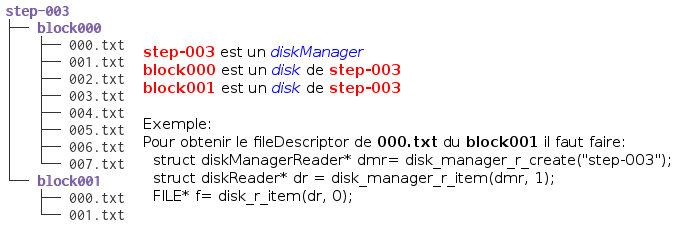
\includegraphics[width=0.8\textwidth]{block.png}

\section{Comment compiler le projet}

\begin{itemize}
	\item make all : Compile tout les fichiers
	\item make test : Lancement de la série de tests automatiques
	\item make doc  : Génération de la documentation (doxygen)
	\item make rapport : Génération du rapport (latex)
	\item make clean : Nettoyage du projet (supression des objets et binaires)
	\item make demo-tp1 : Lancer la démo tp1
	\item make demo-tp2 : Lancer la démo tp2
	\item make demo-tp3 : Lancer la démo tp3
	\item make demo-tp4 : Lancer la démo tp4
	\item make demo-tp5 : Lancer la démo tp5
  \item make demo-tp6 : Lancer la démo tp6
  \item \colorbox{yellow}{make demo-tp7 : Lancer la démo tp7 (Nouveau)}
	\item make rm-rs : Supprime le fichier res/RS.txt et res/disk/RS.txt
  \item make gen-tp5 : Génération de R pour tp5
  \item make gen-tp6 : Génération de R et S pour tp5
  \item \colorbox{yellow}{make gen-tp7 : Génération de R pour tp7 (Nouveau)}
\end{itemize}

\section{Arborescence}

\begin{itemize}
\item bin : Binaire exécutable
\begin{itemize}
  \item demo : Exécutable de démonstration
  \item test : Exécutable de test
\end{itemize}
\item doc : Documentation doxygen sous differents formats
\item rapport : Source du rapport
\item res : Ressources necessaire au projet (fichier de bdd)
\item script  : Script utilisé pour les test
\item src : Source du projet
\begin{itemize}
  \item bdd   : Source de la bibliothéque
  \item demo  : Sources des differentes démonstrations d'utilisation
  \item test  : Sources des dufferents tests
\end{itemize}

\item sujet.pdf  : Sujet du projet
\item README.md  : Le readme du projet
\item rappot.pdf : C'est moi
\item refman.pdf : Documentation format pdf
\end{itemize}

\section{Caracteristiques}

\begin{itemize}
	\item Le code est organisé
	\item Il y a des code des tests
	\item Il y a la doc
	\item Il y a un rapport
	\item Et il y a pleins d'autre chose
\end{itemize}

\section{Démonstration}

Les sources de demosntration sont diponible dans: src/demo
Les exécutables de test sont généré dans: bin/demo
La commande make pour lancer les demo sont: make demo-tp1, make demo-tp2, make demo-tp3 etc...

\begin{itemize}
  \item tp1-natural-join: Natural join R et S
  \item tp2-merge-join-without-duplicate: Merge join sans duplication
  \item tp3-merge-join-with-duplicate: Merge join avec duplication
  \item tp4-hash-join : Hash join
  \item tp5-nested-loop-disk: Nested loop sur disque
  \item tp6 nested loop join + hash join
  \item \colorbox{yellow}{tp7-disk-sort-merge (Nouveau)}
\end{itemize}

\section{Test unitaire}

Les sources de test sont diponible dans: src/test
Les exécutables de test sont généré dans: bin/test
Le script de test est dans script/test.sh
La commande make pour lancer les test est: make test

\begin{itemize}
  \item 00-storeFileBuffer: Ecriture d'un buffer dans un fichier
  \item 01-natural-join-1: Natural join R et S
  \item 02-natural-join-2: Natural join S et R
  \item 03-buf-quick-sort: Fonction de trie d'un buffer
  \item 04-merge-join-without-duplicate-1: Merge join sans duplication R et S
  \item 05-merge-join-without-duplicate-2: Merge join sans duplication S et R
  \item 06-merge-join-with-duplicate-1: Merge join avec duplication R et S
  \item 07-merge-join-with-duplicate-2: Merge join avec duplication S et R
  \item 08-hash-put-equilibre : Test ajout equilibré dans une table de hash
  \item 09-hash-put-desequilibre : Test ajout déséquilibré dans une table de hash
  \item 10-hash-full : Test remplissage complet dans une table de hash
  \item 11-hash-get : Test recupreration d'une entrée dans la table de hash
  \item 12-hash-remove : Test supression / rehash dans une table de hash
  \item 13-hash-join : Test hash join
  \item 14-buffer-read-file: test la lecture avec un buffer extended
  \item 15-buffer-read-file-2: test la lecture avec un buffer extended
  \item 16-disk-buffer-dump: test la lecture d'un disque
  \item 17-disk-nested-loop-r-to-s-test: test le nested loop sur disque r to s
  \item 18-disk-nested-loop-s-to-r-test: test le nested loop sur disque s to r
  \item 19-buffer-decimal
  \item 20-table-puts
  \item 21-disk-block-hash-join
  \item \colorbox{yellow}{22-diskManagerReader (Nouveau)}
  \item \colorbox{yellow}{23-disk-sort-merge (Nouveau)}
\end{itemize}

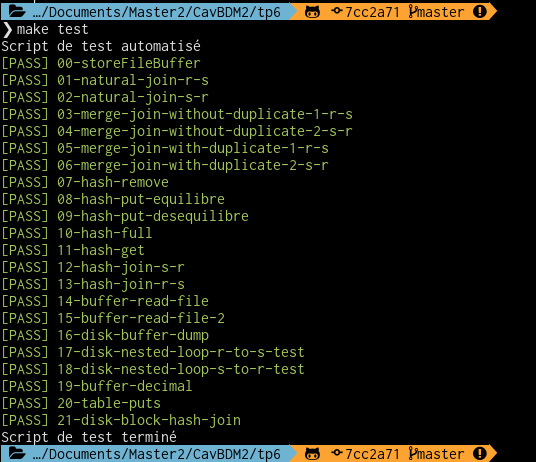
\includegraphics[width=0.8\textwidth]{test.png}

\end{document}
